\begin{frame}[plain]
    \begin{center}
        \vspace{48pt}
        {\huge\bf Faboのセンサーを使ってみよう}
    \end{center}
\end{frame}

\begin{frame}
    \frametitle{Fabo}
    \begin{center}
        \begin{columns}
            \begin{column}{0.6\textwidth}
                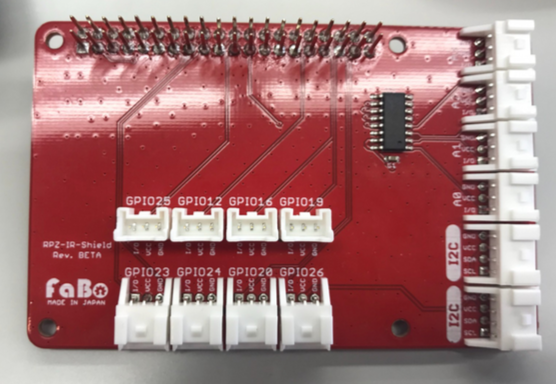
\includegraphics[width=0.6\textwidth]{images/chap05/text05-img004.png}
                {\\シールド}
            \end{column}
            \begin{column}{0.4\textwidth}
                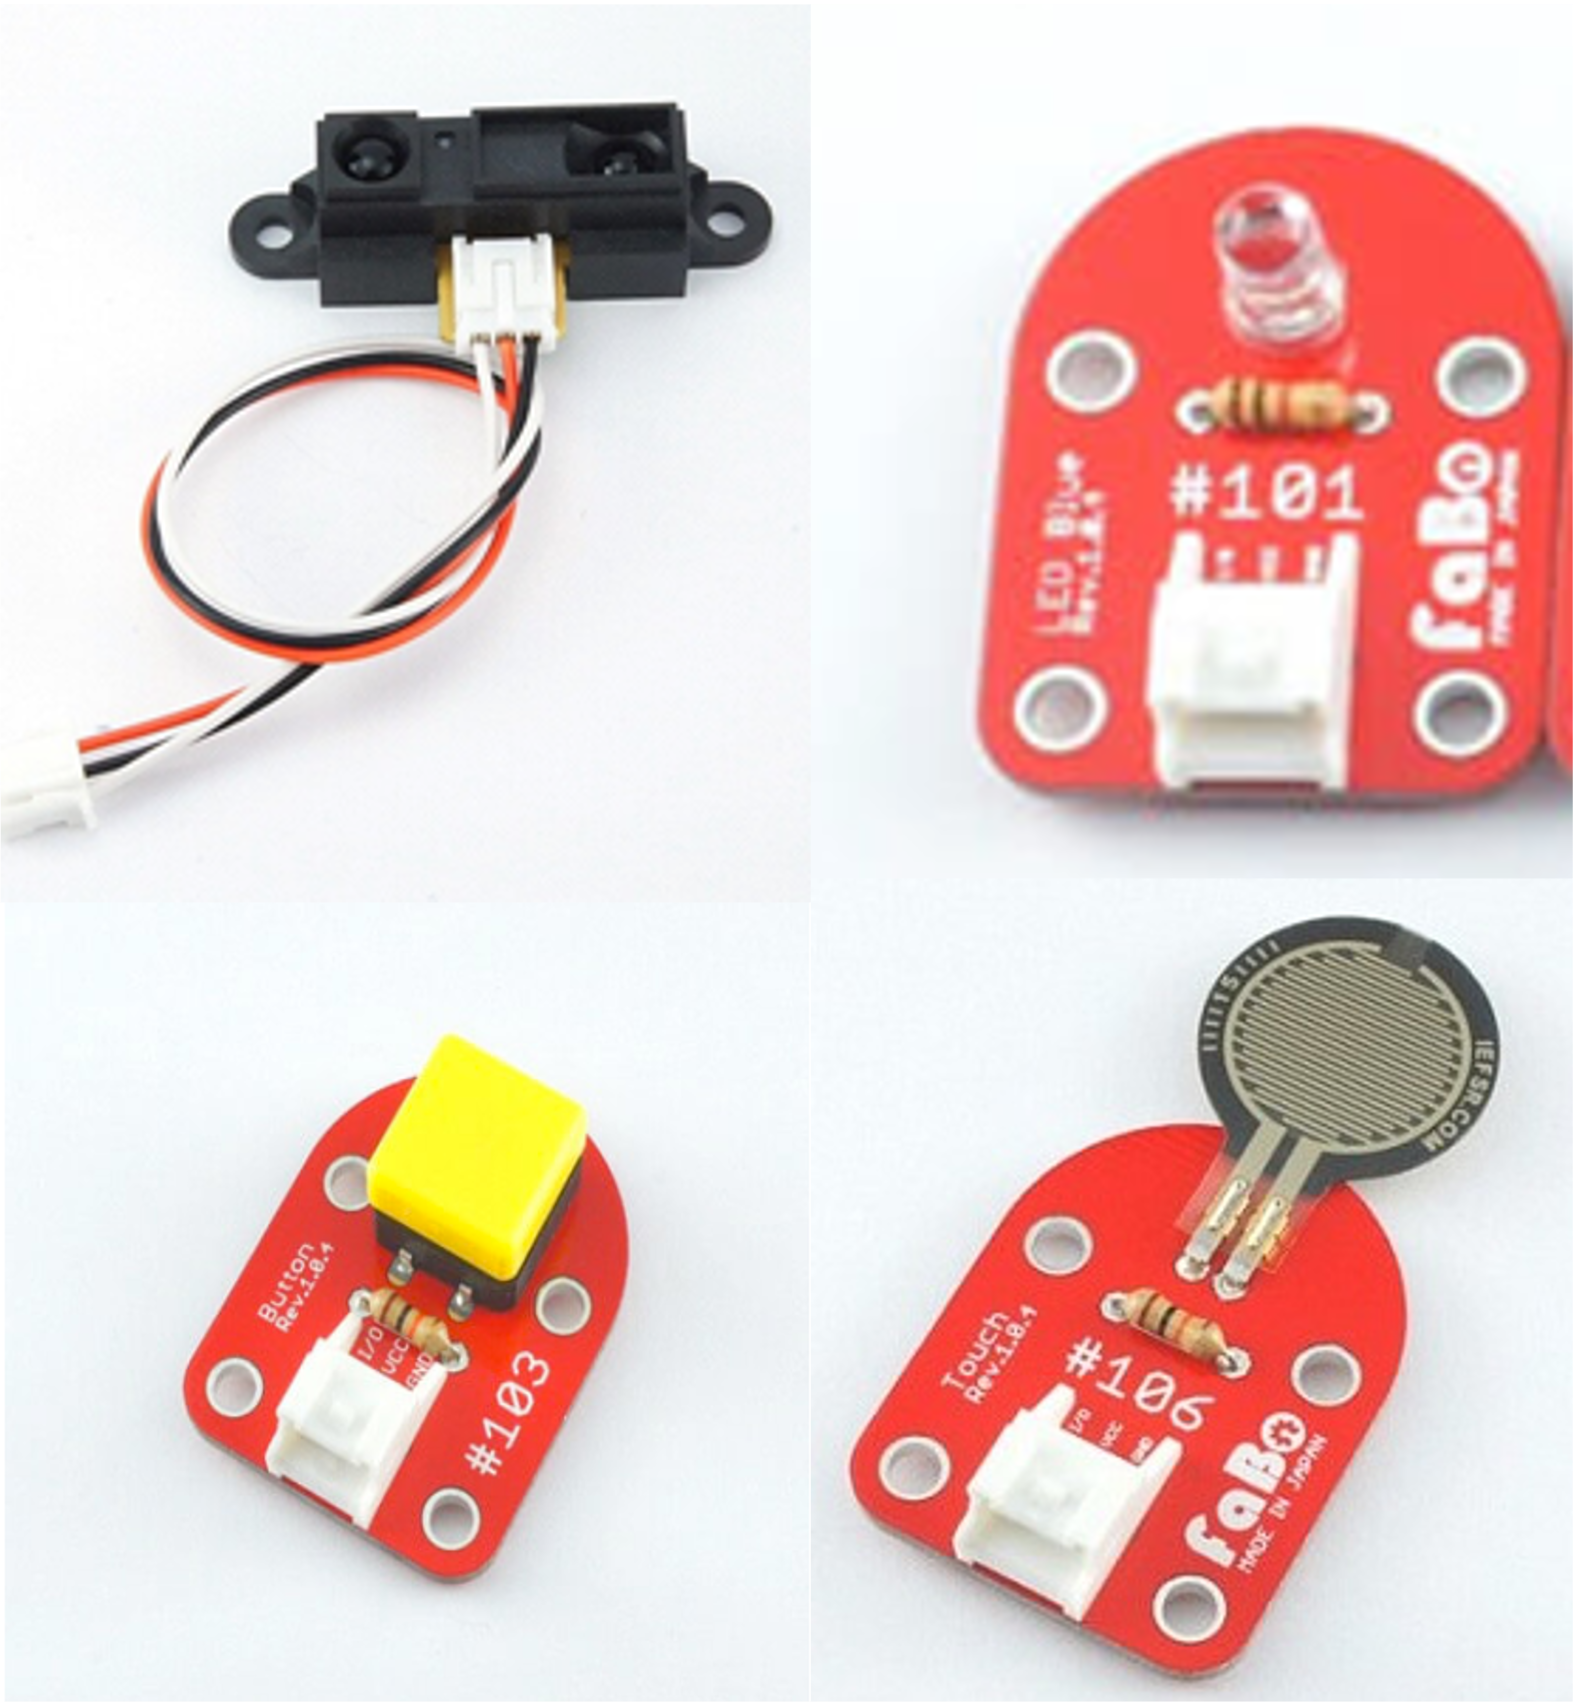
\includegraphics[width=\textwidth]{images/slide/bricks.png}
                {\\ブリック}
            \end{column}
        \end{columns}
        {FaBoのシールドとセンサーは必要な配線がすでにされているから
        自分でどう線をつながなくても簡単にセンサーが使えるよ!} 
    \end{center}
    \textpageref{4}
\end{frame}

\begin{frame}
    \frametitle{シールドを取り付けよう}
    \begin{center}
        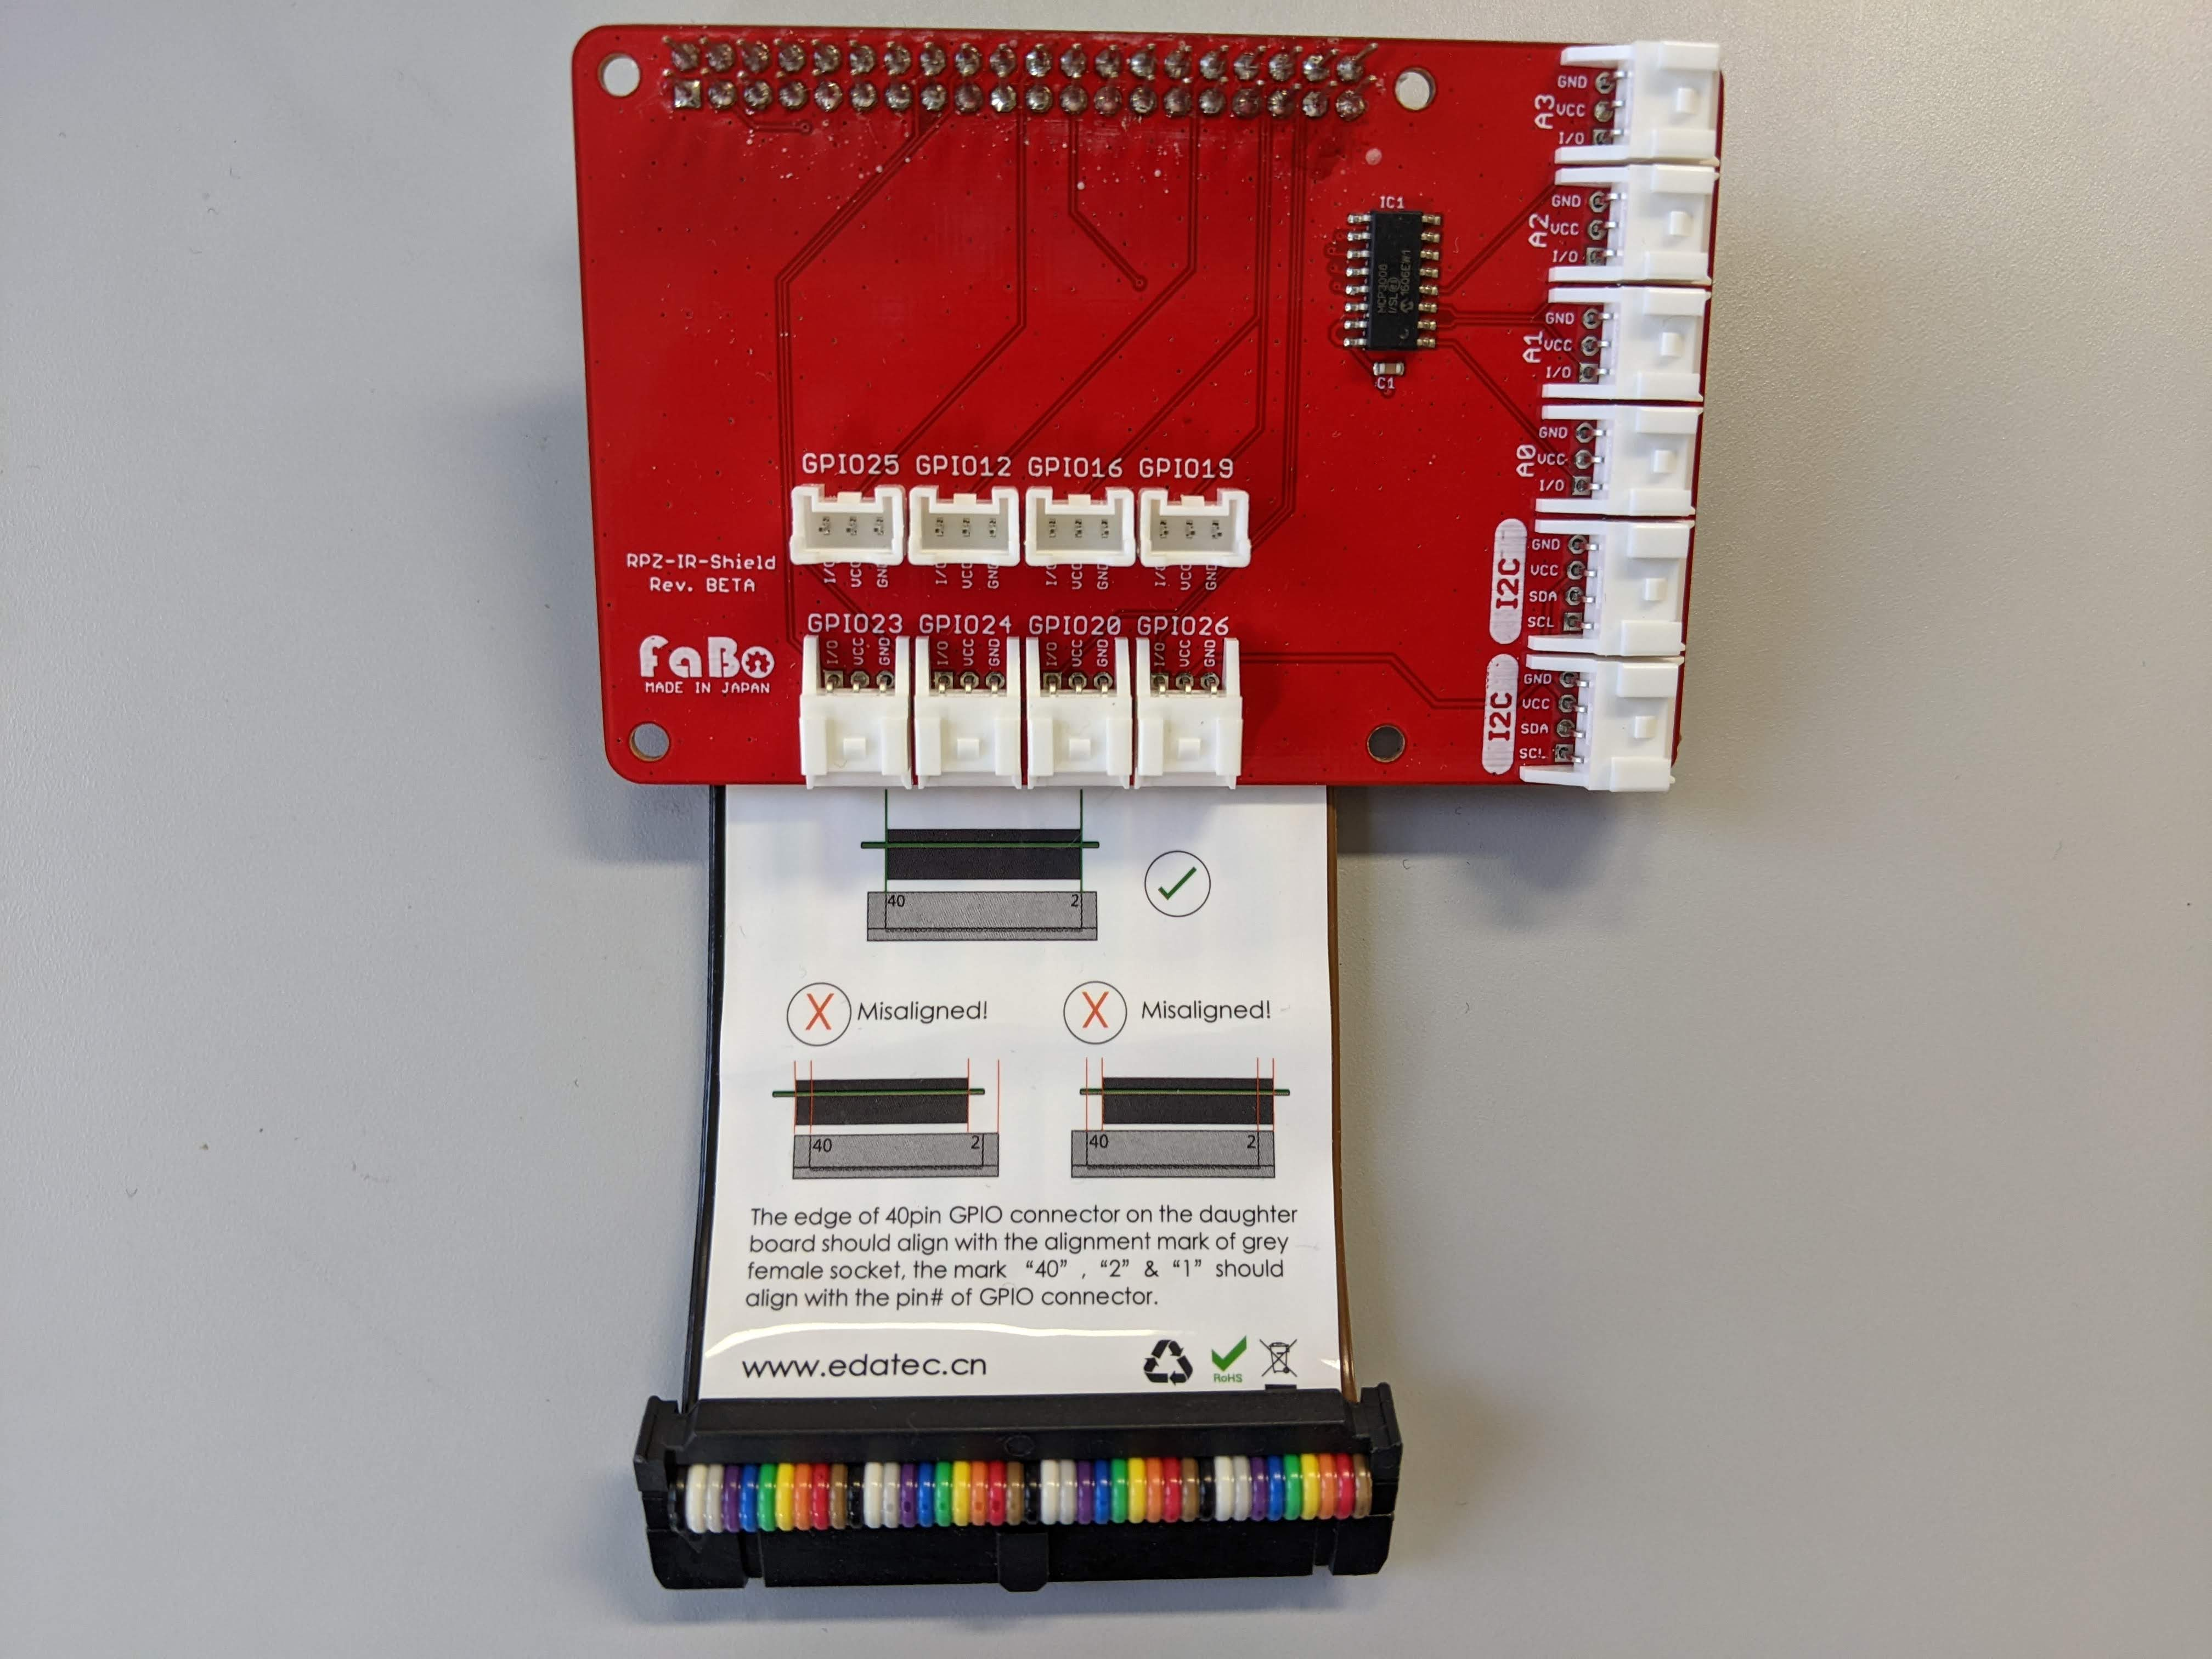
\includegraphics[width=0.6\textwidth]{images/chap05/fabo_and_cable.jpg}
        {\\\color{red}電源を切ってから\color{black}、シールドを取り付けましょう}
    \end{center}
    \textpageref{4}
\end{frame}

\begin{frame}
    \frametitle{\makebox[50pt][l]{\ruby{入力装置}{にゅう|りょく|そう|ち}}}
    \begin{center}
        {コンピュータに信号を送る}
        \begin{itemize}
            \item \ruby{傾斜}{けい|しゃ}センサー
            \item スイッチ
            \item リミットスイッチ
            \item 感圧センサー
            \item ボリューム
            \item \ruby{距離}{きょ|り}センサー
            \item \ruby{照度}{しょう|ど}センサー 
        \end{itemize}
    \end{center}
    \textpageref{6}
\end{frame}

\begin{frame}
    \frametitle{\makebox[50pt][l]{\ruby{出力装置}{しゅつ|りょく|そう|ち}}}
    \begin{center}
        {コンピュータから信号を受け取る}
        \begin{itemize}
            \item LED
            \item \ruby{振動子}{しん|どう|し}
            \item 有機ELディスプレイ
        \end{itemize}
    \end{center}
    \textpageref{6}
\end{frame}

\begin{frame}
    \frametitle{ピン番号}
    \begin{center}
        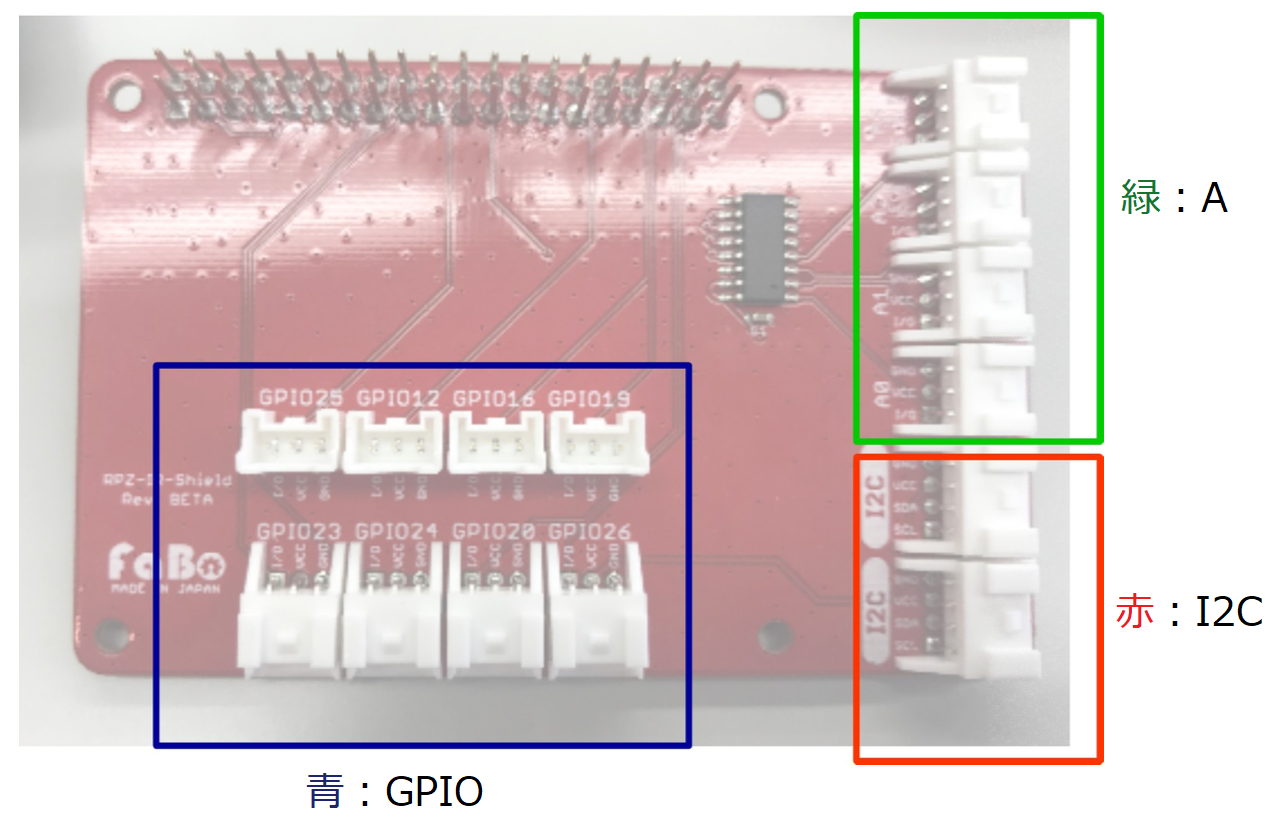
\includegraphics[width=0.6\textwidth]{images/chap05/text05-img012.png}
        \begin{itemize}
            \item A: アナログセンサー用
            \item I2C: 特別な通信用
            \item GPIO: デジタルセンサー用
        \end{itemize}
    \end{center}
    \textpageref{7-8}
\end{frame}

\begin{frame}
    \frametitle{ケーブル}
    \begin{center}
        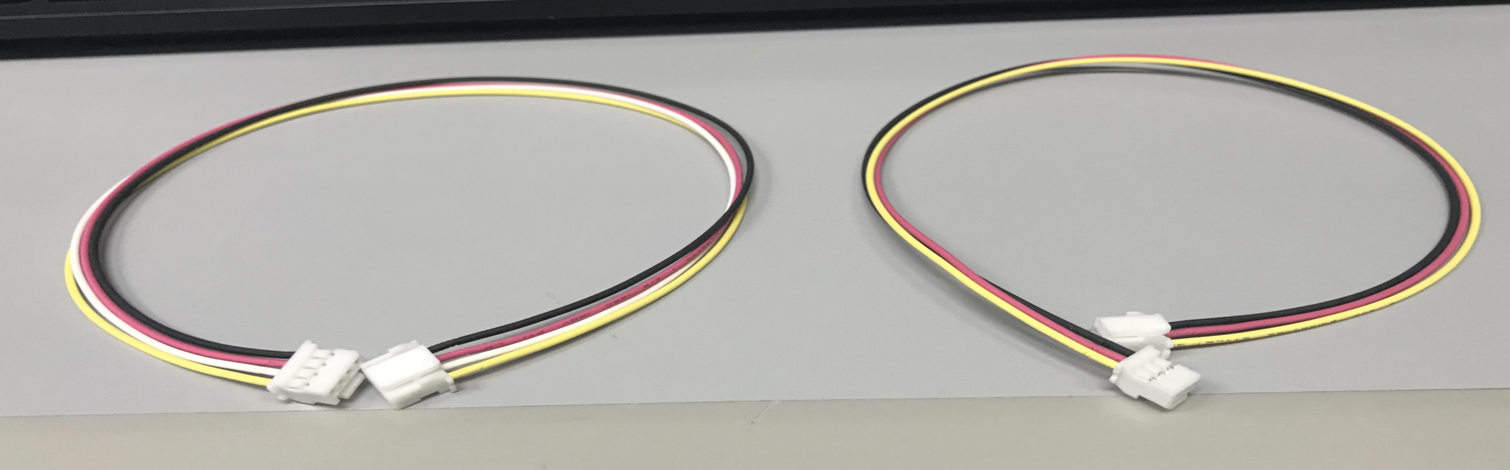
\includegraphics[width=0.6\textwidth]{images/chap05/text05-img013.png}
        \vspace{3pt}
        {\\4ピンケーブルと3ピンケーブルの2種類がある}
    \end{center}
    \textpageref{8}
\end{frame}

\begin{frame}
    \frametitle{ブリックとシールドの接続} 
    \begin{columns}
        \begin{column}{0.48\textwidth}
            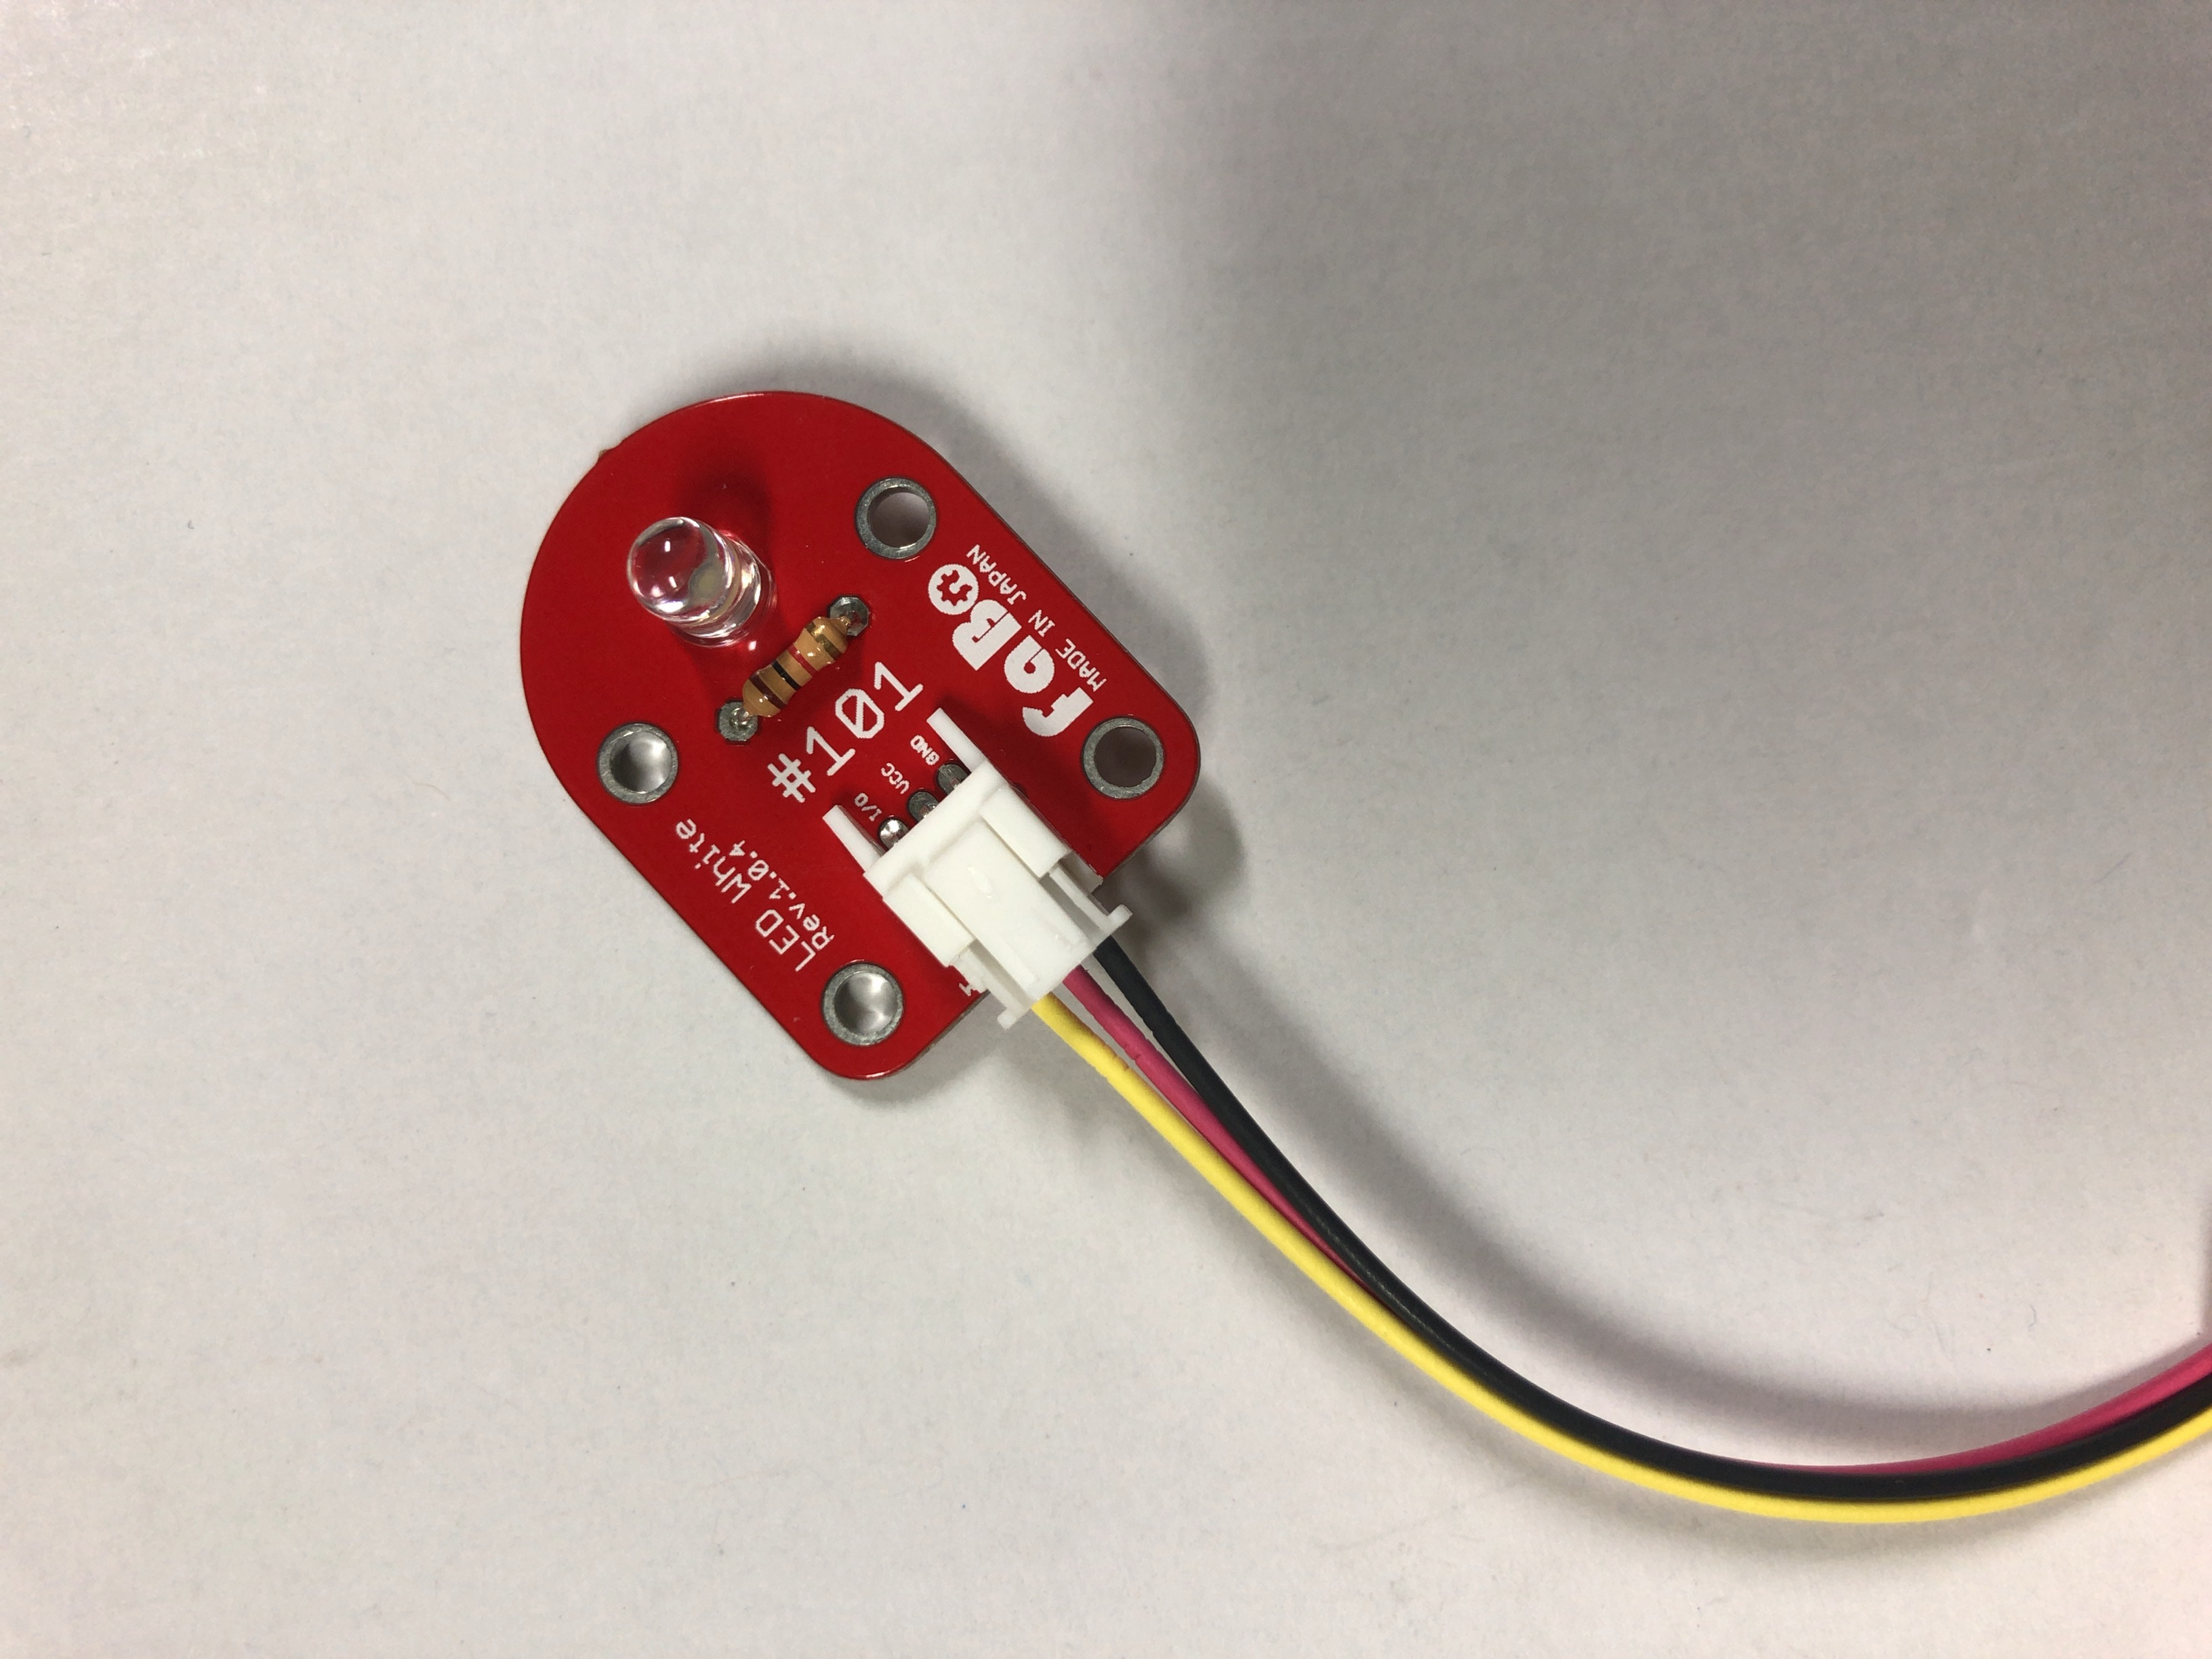
\includegraphics[width=\textwidth]{images/chap05/text05-img008.jpg} 
            {ブリックとケーブル}
        \end{column}
        \begin{column}{0.48\textwidth}
            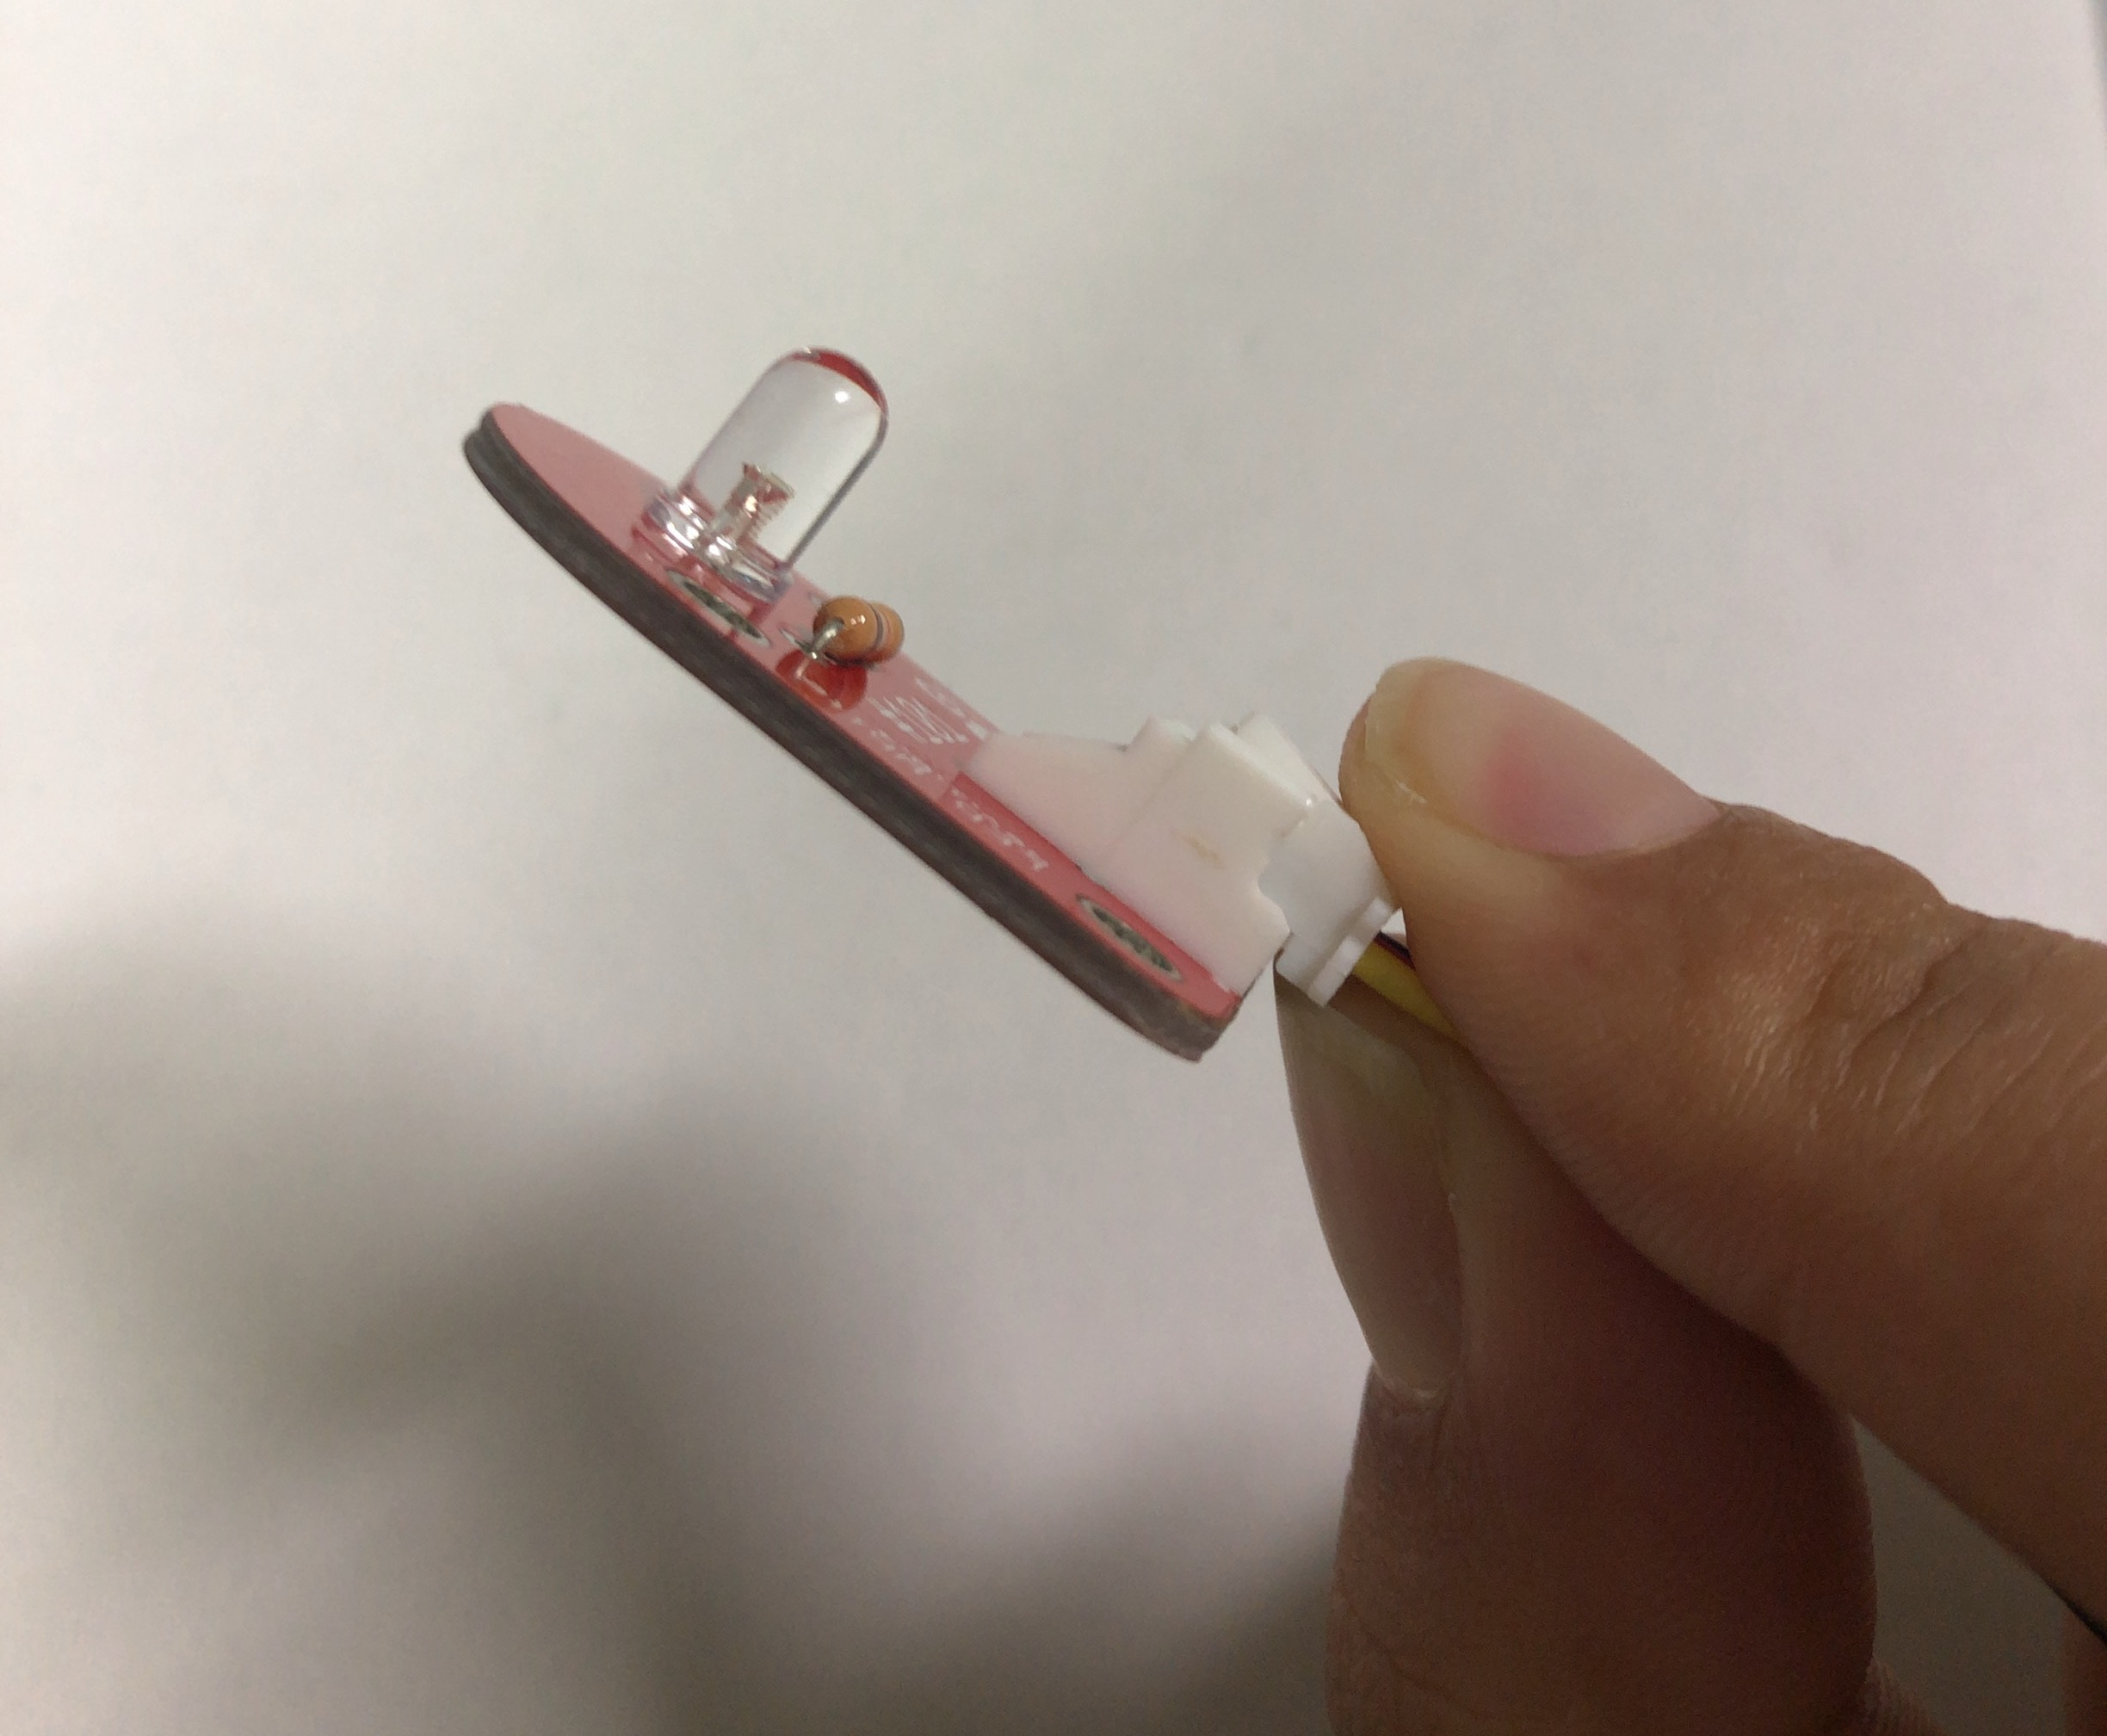
\includegraphics[width=\textwidth]{images/chap05/text05-img011.jpg} 
            {ケーブルとシールド}
        \end{column}
    \end{columns}
    \textpageref{5}
\end{frame}

\begin{frame}
    \frametitle{ブリックとシールドの取り外し}
    \begin{center}
        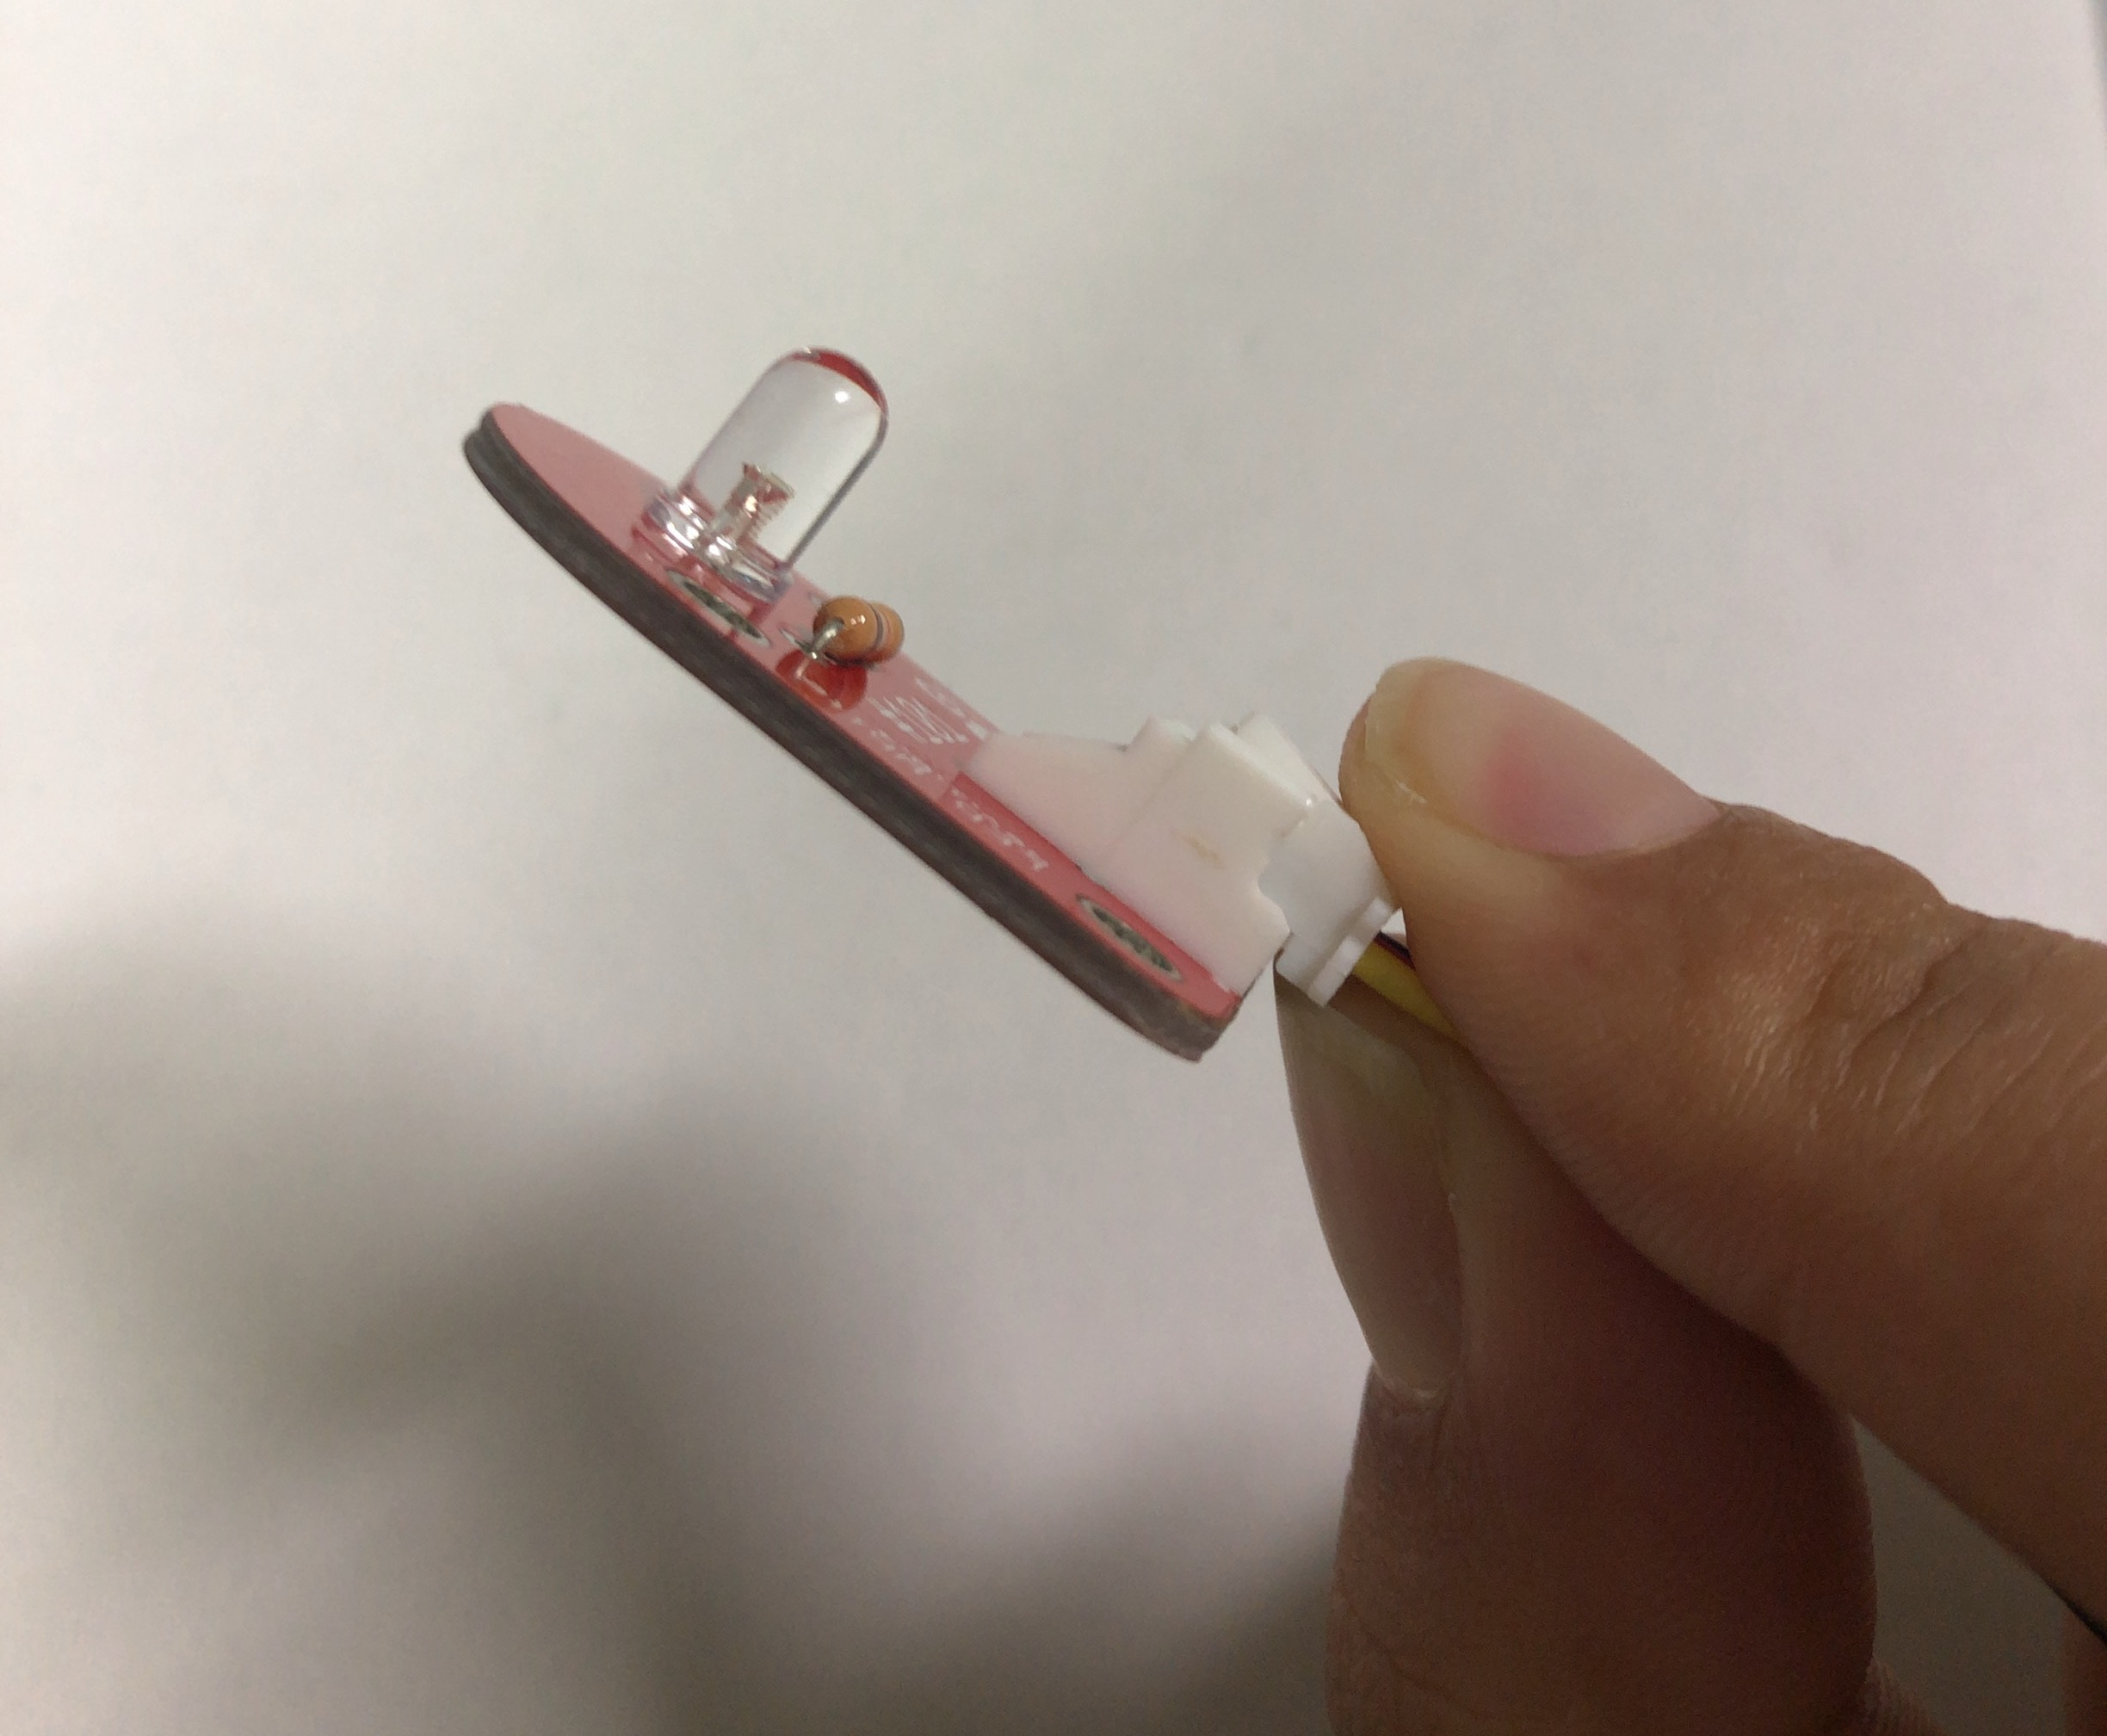
\includegraphics[width=0.6\textwidth]{images/chap05/text05-img011.jpg}
        {\\つめを押して抜く}
    \end{center}
    \textpageref{6}
\end{frame}

\begin{frame}[fragile]
    \begin{exampleblock}{問題を解いてみよう}
        \begin{itemize}
            \item 教科書6ページ 問題5-2(1問)
            \item 教科書7ページ 問題5-3(1問)
        \end{itemize}
    \end{exampleblock} 
\end{frame}
